\documentclass[journal]{vgtc}                % final (journal style)
%\documentclass[review,journal]{vgtc}         % review (journal style)
%\documentclass[widereview]{vgtc}             % wide-spaced review
%\documentclass[preprint,journal]{vgtc}       % preprint (journal style)
%\documentclass[electronic,journal]{vgtc}     % electronic version, journal

\let\ifpdf\relax

%% Uncomment one of the lines above depending on where your paper is
%% in the conference process. ``review'' and ``widereview'' are for review
%% submission, ``preprint'' is for pre-publication, and the final version
%% doesn't use a specific qualifier. Further, ``electronic'' includes
%% hyperreferences for more convenient online viewing.

%% Please use one of the ``review'' options in combination with the
%% assigned online id (see below) ONLY if your paper uses a double blind
%% review process. Some conferences, like IEEE Vis and InfoVis, have NOT
%% in the past.

%% Please note that the use of figures is not permitted on the first page
%% of the journal version.  Figures should begin on the second page and be
%% in CMYK or Grey scale format, otherwise, colour shifting may occur
%% during the printing process.  Papers submitted with figures on the
%% first page will be refused.

%% These three lines bring in essential packages: ``mathptmx'' for Type 1
%% typefaces, ``graphicx'' for inclusion of EPS figures. and ``times''
%% for proper handling of the times font family.

\usepackage{mathptmx}
\usepackage{graphicx}
\usepackage{times}

\usepackage{pbox}

%% We encourage the use of mathptmx for consistent usage of times font
%% throughout the proceedings. However, if you encounter conflicts
%% with other math-related packages, you may want to disable it.

%% If you are submitting a paper to a conference for review with a double
%% blind reviewing process, please replace the value ``0'' below with your
%% OnlineID. Otherwise, you may safely leave it at ``0''.
\onlineid{0}

%% declare the category of your paper, only shown in review mode
\vgtccategory{Research}

%% allow for this line if you want the electronic option to work properly
\vgtcinsertpkg

%% In preprint mode you may define your own headline.
%\preprinttext{To appear in an IEEE VGTC sponsored conference.}

%% Paper title.

\title{The impact of user interface design of eco-feedback systems on consumer behavior}

%% This is how authors are specified in the journal style

%% indicate IEEE Member or Student Member in form indicated below
\author{Aur\'{e}lie Fakambi and Wouter Menninga}
\authorfooter{
%% insert punctuation at end of each item
\item
  A. Fakambi is a Computing Science Master student at the University of Groningen, E-mail: A.Fakambi@student.rug.nl.
\item
  W. Menninga is a Computing Science Master student at the University of Groningen, E-mail: W.G.Menninga@student.rug.nl.
}

%% A teaser figure is NOT to be included.

%other entries to be set up for journal
%\shortauthortitle{Biv \MakeLowercase{\textit{et al.}}: Global Illumination for Fun and Profit}
%\shortauthortitle{Firstauthor \MakeLowercase{\textit{et al.}}: Paper Title}

%% Abstract section.
\abstract{Saving energy in buildings has become and remains a major issue for the planet.% AURELIE COMMENT : WHY IS IT AN ISSUE AND A CHALLENGE ?
The last decade, systems have been developed to provide consumers with information about their energy consumption. 
Research has shown that the type of information displayed and the techniques used to present it have an impact on the user energy saving. This raises the question about how to display the information to the consumer in a comprehensive, attractive and non-intrusive way. \\

In this paper we compare and discuss the various methods of visualizing energy usage for consumers. Some of the design components of user interfaces such as historical comparisons and presentation of costs are more likely to aid in providing the consumer with an understanding of his energy usage and changing his behavior.
We will extract the most effective methods from research and surveys. \\

The comparison of the different methods is based on the reduction of energy usage of consumers using such eco-feedback systems and if consumers keep using the eco-feedback systems for longer periods of time.

Little work has been done in the design of eco-feedback systems. We expect to find the most effective methods to visualize energy consumption data for future eco-feedback systems.
% AURELIE COMMENT ADD THE RESULTS - We can conclude that design components such as historical comparison,presentations of corsts are the most effective ones, they increase the users awareness.
} % end of abstract

%% Keywords that describe your work. Will show as 'Index Terms' in journal
%% please capitalize first letter and insert punctuation after last keyword
\keywords{Eco-Feedback, interface design, energy consumption, consumption feedback systems, energy feedback}

%% ACM Computing Classification System (CCS). 
%% See <http://www.acm.org/class/1998/> for details.
%% The ``\CCScat'' command takes four arguments.

\CCScatlist{ % not used in journal version
  \CCScat{K.6.1}{Management of Computing and Information Systems}%
{Project and People Management}{Life Cycle};
  \CCScat{K.7.m}{The Computing Profession}{Miscellaneous}{Ethics}
}

\manuscriptnote{~}

%% Copyright space is enabled by default as required by guidelines.
%% It is disabled by the 'review' option or via the following command:
% \nocopyrightspace

%%%%%%%%%%%%%%%%%%%%%%%%%%%%%%%%%%%%%%%%%%%%%%%%%%%%%%%%%%%%%%%%
%%%%%%%%%%%%%%%%%%%%%% START OF THE PAPER %%%%%%%%%%%%%%%%%%%%%%
%%%%%%%%%%%%%%%%%%%%%%%%%%%%%%%%%%%%%%%%%%%%%%%%%%%%%%%%%%%%%%%%%

\begin{document}

%% The ``\maketitle'' command must be the first command after the
%% ``\begin{document}'' command. It prepares and prints the title block.

%% the only exception to this rule is the \firstsection command
\firstsection{Introduction}

\maketitle

%% \section{Introduction} %for journal use above \firstsection{..} instead

% problem of energy usage
Reducing energy usage in buildings still remains a major challenge.

One method of reducing energy consumption is by increasing the awareness of consumers about their energy consumption using eco-feedback systems. These are systems with integrated sensors that provide the consumers in the building with information about their energy usage. The goal is that this leads to more energy efficient behavior by the consumers in the building. 

However, research has shown that the type of information displayed and the technique used to present it have an impact on the user behavior.
For example, studies have demonstrated that the information provided must be intuitive, clear and simple and the UI attractive and not too intrusive (e.g. not too many notifications) so that the users keep using it and is integrated in their everyday life\cite{spagnolli2011eco}.

This means that the design of the user interface is a key factor in changing the user's energy consumption behavior and raises the question of what the most effective methods to visualize energy consumption data for future eco-feedback systems are. 

% to be corrected ?
Our goal is to investigate the different ways to display to the users their electricity usage.
The main UI components of eco-feedback systems are: historical comparison, presentation of costs, incentive, reward and commitment. From those components we want to extract the most effective ones: the ones which are more likely to help users save energy. 

% to be corrected ?
Based on previous surveys we are going to compare the effectiveness of different eco-feedback systems by comparing the reduction in electricity usage. Additionally, we will combine the results/responses of surveys and interviews with users of such eco-feedback systems, to assess the effectiveness of different UI components. 

% AURELIE COMMENT , rephrase:
We aim at answering many questions in our paper, many decisons has to be made when designing such systems : \\
\textbf{what type of data} should be displayed ? \\
\textbf{how} should the data be displayed to users ? \\
\textbf{which time scale} should be chosen to display those data ? 

In the first part the design components will be presented, in a second part surveys and in the third part our conclusion % To be improved

%to find the most effective methods to visualize energy consumption data for future eco-feedback systems.

% 'integrating sensors and systems to create eco feedback systems' which provide people in building with information about energy consumption behavior 
% many studies have shown that feedback works effectively...[ref]
%It has been shown in many studies that feedback systems have effect in reducing energy consumption
% design of user interface is a key factor to have impact on energy behavior
\section{User Interface components}
Developers have been implementing different types of applications: classical eco-feedback systems or either serious games (eg. games which the purpose isn't just entertainment) %( ex *** ) 
to make it even more attractive to the users and increase their commitment.

\subsection{Displays}
These eco-feedback systems are available on smart meter, personal computer, mobile devices and house/wall displays. %TODO what is better?? 
% AURELIE COMMENT : should we have a part only for the displays

Important aspects of eco-feedback systems are the kind of information displayed and the method of display. However, the aesthetics are also relevant for the engagement, pleasure and interest of the user\cite{bartram2015design}.

In most of the eco-feedback systems some design components are often encountered.
In this part they will be defined and later we will discuss their effect on users changing behavior in order to elect the most effectives ones. 
%Feedback
%Three types : Direct
%Indirect
%Inadvertent
%Presentation of costs

\subsection{Comparison}
Two types of comparison are often presented in eco-feedback systems: historical and normative.
Historical comparison is defined as the ability of users to view their current consumption compared to their past consumption. %SOURCE
The historical comparison can often be displayed on a daily, weekly, monthly or yearly basis. It is used in the majority of eco-feedback systems, because it can be easily understood by the users, especially thanks to the use of bar charts (cf part BLABLABLA). Observing those graphs helps them reminding their behavior (why they used more energy this particular day for example) and in consequence change their bad habits.

Most eco-feedback systems do not take into account factors such as weather (household use more energy when it is colder) or households leaving for vacation when establishing the historical comparison\cite{karjalainen2011consumer}. This means that absolute values are analyzed whereas they should have been normalized first. Some improvements in the eco-feedback systems take those fluctuations and changes into account for more accuracy and consistency.

%The historical comparison deals with comparison with the household's own prior consumption 
Another type of comparison is the normative one, which deals with comparison at a local, regional level or in a neighborhood. The effectiveness of the normative comparison comes from the fact that users are influenced by social norms and pressure. Seeing, for example, that their neighbors consume less energy than they do should encourage them to do the same. It has been seen in previous research that such normative comparisons can lead to significant reductions in electricity usage\cite{peschiera2010response,siero1996changing,iyer2006comparison}.

%We will see in the Survey section that the historical comparison is the most effective one.

\newpage
\subsection{Goal setting}
Environmental psychology departments have demonstrated that users need to find motivation in order to change their behavior. Some eco-feedback systems provide goal settings design components: the users can set the goal themselves or they come from the software itself or the community of users of the eco-feedback system.  %AURELIE new :
One way to generate goal setting is to calculate a baseline of energy consumption based on past usage and then set the goal as some percentage reduction from the baseline. % the computation of this baseline won't be presented in here
An example of a goal could be: "reduce your energy consumption with 5\% compared to the previous month".

Every household consumes in a different way. Therefore, households in the same neighborhood are not likely to have the same goals.


Eco-feedback systems can aid users to reach their goal thanks to tips and advices.
To create an energy saving positive dynamic the eco-feedback system should reward their users when they reach their goal. 

\subsection{Disaggregation or appliance specific breakdown}
Disaggregation or appliance-specific breakdown allows consumers to have a better understanding about which appliance consumes what so it is easier for them to change a particular behavior. It helps consumers to understand the impact of a specific behavior or the use appliance to answers questions like ``if I let the TV on for 5 hours, how much do I consume?".
%However this design component is C'est toujours à l'étape de recherche because installing and maintaining individual sensors is difficult.

\subsection{Reward \& penalization / incentives}
Rewards and penalization allow users to earn rewards if they reduce their energy consumption or in the contrary to be penalized if they waste energy. A system of rewards and penalization encourages behavior that leads to energy conservation and discourage wasteful behavior.

The incentive design component is related to the rewards \& penalization design components. Users can be rewarded in a financial or non-financial way. Financial incentives can be credit on a electricity bill and non financial incentives can be prices such as an energy efficient lamp or reaching higher levels in the game.
Previous research \cite{petersen2007dormitory} has shown that incentives can result in significant electricity use reductions.

\section{Presentation of the information inside the components : graphical, numerical and textual presentation} % Neeeed a better title
In this section the following questions will be answered : What is the best and most effective way to present the information inside the key design components identified in the previous part ? What do the users understand easily texts or graphs ?
%Kind of presentation that the users prefere graphical vs Text => guidelines of Smith and Mosier
%More information about the chart pie, bar chart, tabular presentation understanding among users.

\section{The Surveys}
Several studies researching the effectiveness of consumer feedback on electricity consumption have been done before in order to get a better understanding of what the users wants to see and to help him. % BLABLABLA, user-centered perspecive
This section will discuss the results of some of these studies. \\
% In this part four surveys and their results will be presented. The surveys can be divided in two parts: the ones who try to define the users wishes, and the ones where the users compare different design components.
% User-wishes surveys
% Protoypes surveys

% For each survey we need to analyse
\subsection{User wishes surveys}
In this subsection BLABLABLABLA

\subsection{Comparison/comparative surveys} %better title to be found
In this subsection BLABLABLABLA

In a study from S. Karjalainen\cite{karjalainen2011consumer} from 2010, interviewing and paper prototyping were used to find the best ways to present information for maximum energy reductions. In this study, interviews with consumers were held to find out about their attitude towards energy monitoring and what kind of feedback they understand and prefer.

The qualitative interviews showed that 8 out of 14 interviewees actively try to save electricity at home, while all 14 responded they want to monitor electricity consumption. The interviewees also indicated that they prefer to receive feedback via a bill, web page or dedicated wall display rather than a mobile phone. \\

Additionally, 8 paper user interface prototypes were developed. Table~\ref{prototypes} shows an overview of the UI components present in these prototypes.

\begin{table}
%% Table captions on top in journal version
  \caption{Overview of information presented in the different prototypes by Karjalainen\cite{karjalainen2011consumer}}
  \label{prototypes}
  \scriptsize
  \begin{center}
    \begin{tabular}{|l|cccccccc|}
    \hline
      & \multicolumn{8}{|c|}{Prototype} \\
    
      UI component & 1 & 2 & 3 & 4 & 5 & 6 & 7 & 8 \\
    \hline
      Historical comparison & $\times$ &  &  &  &  &  &  & \\ \hline
      Normative comparison &  & $\times$ & $\times$ &  &  &  &  & \\ \hline
      Goal setting &  & $\times$ &  &  &  &  &  & \\ \hline
      Consumption (kWh) & $\times$ & $\times$ &  &  &  & $\times$ & $\times$ & $\times$ \\ \hline
      Power (W) &  &  &  & $\times$ & $\times$ &  &  & \\ \hline
      Costs (Euro) &  & $\times$ &  &  &  & $\times$ &  & \\ \hline
      Environmental factor (kg CO$_2$) &  &  & $\times$ &  &  &  &  & \\ \hline
      Household total & $\times$ & $\times$ & $\times$ & $\times$ & $\times$ & $\times$ & $\times$ & \\ \hline
      Disaggregation day/night &  &  &  &  &  &  & $\times$ & \\ \hline
      Disaggregation by device &  &  &  &  & $\times$ & $\times$ & $\times$ & $\times$ \\ \hline
      Chart & $\times$ &  &  & $\times$ & $\times$ &  & $\times$ & $\times$ \\ \hline
      Other pictorial &  & $\times$ & $\times$ &  &  &  &  & \\ \hline
      Table &  &  &  &  &  & $\times$ &  & \\ \hline
      Other numeric &  & $\times$ & $\times$ &  & $\times$ &  &  & $\times$ \\ \hline
      Textual &  &  & $\times$ &  &  &  &  & \\ \hline
      Chooseable time period &  & $\times$ & $\times$ & $\times$ &  & $\times$ & $\times$ &  $\times$ \\ \hline
    \end{tabular}
  \end{center}
\end{table}

The prototypes were shown to consumers, to find out how well these interfaces are understood by them. The prototypes were displayed to the consumers one by one and after showing all the prototypes, they were asked if they understood the prototypes and asked to choose the prototype they would prefer to use themselves.\\

The results of the survey can be seen in Table~\ref{prototypesresults}. Most prototypes were understood by the participants. Problems with understanding were mostly due to the fact that many people are not familiar with the scientific units used and do not, for example, understand the difference between W and kWh. Secondly, people in general do not understand how CO$_2$ emissions relate to energy consumption.
In contrast, information presented in charts and tables is understood easily by the participants.

% results
\begin{table}
%% Table captions on top in journal version
  \caption{Nr of participants that understood and preferred for each of the prototypes. Total participants: 14.}
  \label{prototypesresults}
  \scriptsize
  \begin{center}
    \begin{tabular}{|lcc|}
    \hline
       & \multicolumn{1}{p{2.5cm}}{\centering Nr of participants that understood prototype} & 
       \multicolumn{1}{p{3cm}|}{\centering Nr of participants who preferred prototype}  \\ \hline
       Prototype 1 & 14 & 1 \\ 
       Prototype 2 & 14 & 1 \\ 
       Prototype 3 & 8 & 0 \\ 
       Prototype 4 & 12 & 0 \\ 
       Prototype 5 & 7 & 1 \\ 
       Prototype 6 & 14 & 7 \\ 
       Prototype 7 & 13 & 1 \\ 
       Prototype 8 & 14 & 3 \\ \hline
    \end{tabular}
  \end{center}
\end{table}

\underline{Analysis}

Participants were also asked some general questions about how important they find certain aspects of eco-feedback systems. The questions were answered using a scale of 1 to 5, where 5 was very important and 1 not important at all. The question with the average of the response of the 14 participants can be seen in Table~\ref{prototypesquestions}.

% results
\begin{table}
%% Table captions on top in journal version
  \caption{General questions about eco-feedback systems}
  \label{prototypesquestions}
  \scriptsize
  \begin{center}
    \begin{tabular}{|ll|}
    \hline
       Question (\textit{How important is it to...}) & Avg. \\ \hline
       \pbox{20cm}{\textit{be able to compare your household's consumption}\\\textit{to other households?}} & 3.6 \\ ~\\[-0.25cm]
       \textit{be able to compare your consumption to your prior consumption?} & 4.4 \\ 
       \textit{have a target level for consumption?} & 3.5 \\ 
       \textit{know the consumption of individual devices?} & 4.1 \\ 
       \textit{receive information on actions which would save energy?} & 3.9 \\
       \hline
    \end{tabular}
  \end{center}
\end{table}

The results of this study by Karjalainen found the following UI components most valued by consumers: presentation of costs, device-specific breakdown of energy usage and historical comparison.
~\\

Research from 2010 by Peschiera et al.\cite{peschiera2010response} provides more insight into the effectiveness of the \textit{normative comparison} component. In their study, they tried to find out if there are differences in energy savings when participants only view personal electricity usage information versus participants also viewing average building occupant usage and usage of peers in their personal network.

To examine if such normalized comparison information motivates electricity-saving behavior, they fitted 83 rooms of a dormitory building in New York City to measure the electricity usage.

They divided the occupants participating in the study into four distinct groups:
\begin{itemize}
\item \textit{Group A} -- ability to view individual historical comparison with past vs. present utilization.
\item \textit{Group B} -- same as group A, but with additional ability to view individual vs. average electricity usage of all other participating occupants.
\item \textit{Group C} -- same as group B, but with additional ability to view electricity usage of peers in that individual's network.
\item \textit{Control Group} -- No access to electricity usage information.
\end{itemize}

At the start of the study, occupants received an email explaining how to access their personal electricity consumption reports. During the study, they received several more notification emails to remind them that their electricity usage report was ready.

Three days after the initial email, the average electricity consumption for Group C was 34\% lower than the consumption of the Control Group and 20\% lower than the consumption in the period before the study.
After sending the second consumption notification email, the average electricity consumption dropped to 45\% below that of the Control Group (28\% less than before the study).
Group B only saw a significant reduction after the second notification email and Group A did not have a significant improvement.

These results show the added value of using electricity consumption data from peer networks (\textit{normalized comparison}) in reducing consumers energy consumption.
~\\

Another study from R.K. Jain et al.\cite{jain2012assessing}, a prototype eco-feedback system was built, with five key design components:
\begin{itemize}
\item \textit{Historical comparison} - ability to view historical electricity consumption in three modes (24h, to date and last week)
\item \textit{Normative comparison} - ability to view the average electricity consumption of friends
\item \textit{Rewards and penalization} - ability to get points or lose points based on consumption behavior
\item \textit{Incentives} - ability to redeem points for prizes
\item \textit{Disaggregation} - ability to find out the consumption of specific devices
\end{itemize}

The prototype was designed to allow users to go to any of the key design components with a single click from the main view.

The system gathered and stored data on logins and use of the system in a database for later analysis.\\

Participants were divided into three groups: one group had access to room-level electricity usage data and consumption information for participants in their peer network added to the historical comparison graphs. 
The second group only had access to the room-level electricity usage data.
The third group was a control group without access to the eco-feedback system.

The researchers formulated and tested three hypothesis, namely:
\begin{enumerate}
\item Users who reduced their energy usage relative to the control group, will have visited the eco-feedback system more often than users who increased or maintained their energy usage.
\item Users that use: historical comparison, normative comparison, incentives/rewards or disaggregation will login more than users that do not use this feature.
\item The sign of the number of reward points a users views on their first login correlates with the number of times a user will log into the eco-feedback system.
\end{enumerate}

In Table~\ref{hypo1}, the results of performing an analysis of the login data can be seen. The data in this table confirms the hypothesis that users who decreased consumption logged in more often (almost twice as often) than users with an increased consumption. \\

\begin{table}
%% Table captions on top in journal version
  \caption{The results for the first hypothesis}
  \label{hypo1}
  \scriptsize
  \begin{center}
    \begin{tabular}{cccc}
    \multicolumn{1}{p{1cm}}{\centering } &
       \multicolumn{1}{p{2.5cm}}{\centering Users who reduced consumption} &
       \multicolumn{1}{p{2.5cm}}{\centering Users who increased consumption} &
       \multicolumn{1}{p{1cm}}{\centering p-value} \\
    \hline
      Mean user logins &  5.13 & 2.60 & .028\\

    \end{tabular}
  \end{center}
\end{table}

Table~\ref{hypo2} shows the correlation between logins and use of specific design components. From these results, it can be concluded that users who used the \textit{historical comparison} feature, on average logged in 3 more times that users that did not use that feature. Additionally, users that used the \textit{incentives} feature logged in more that 3 additional times compared to users that did not use that feature.

For the \textit{normative comparison} and \textit{disaggregation} features, the p-value is not significantly low to reject the null hypotheses. \\

\begin{table}
  \caption{Correlation between user logins and the use of specific design components}
  \label{hypo2}
  \scriptsize
  \begin{center}
    \begin{tabular}{lccc}
    \multicolumn{1}{p{2.5cm}}{\centering Mean user logins by component used} &
       \multicolumn{1}{p{2cm}}{\centering Users who used feature} &
       \multicolumn{1}{p{2cm}}{\centering Users who did not use feature} &
       \multicolumn{1}{p{1cm}}{\centering p-value} \\
    \hline
      Historical comparison &  4.61 & 1.67 & .0009\\
      Normative comparison &  5.00 & 2.40 & .12\\
      Incentives/rewards &  4.49 & 1.25 & .0001\\
      Disaggregation &  4.60 & 4.00 & .64\\

    \end{tabular}
  \end{center}
\end{table}

In Table~\ref{hypo3}, the results for the third hypothesis can be seen. Users who viewed a positive number of points on their first login, logged in 2.5 more times than users that got to see a negative number of points on their first login. \\

\begin{table}
  \caption{Correlation between the sign of the number of points on first visit and number of logins}
  \label{hypo3}
  \scriptsize
  \begin{center}
    \begin{tabular}{lccc}
    \multicolumn{1}{p{2cm}}{\centering } &
       \multicolumn{1}{p{2cm}}{\centering Users that viewed positive points} &
       \multicolumn{1}{p{2cm}}{\centering Users that viewed negative points} &
       \multicolumn{1}{p{1cm}}{\centering p-value} \\
    \hline
      Mean user logins &  4.79 & 2.10 & .0059\\

    \end{tabular}
  \end{center}
\end{table}


In another paper, Erickson et al.\cite{erickson2013dubuque} build a city-scale eco-feedback system aimed at reducing electricity consumption. The system provided households with fine-grained feedback about the electricity usage and has incentives, comparisons and goal setting for encouragement to save energy. \\

\begin{figure}[h]
	\centering
	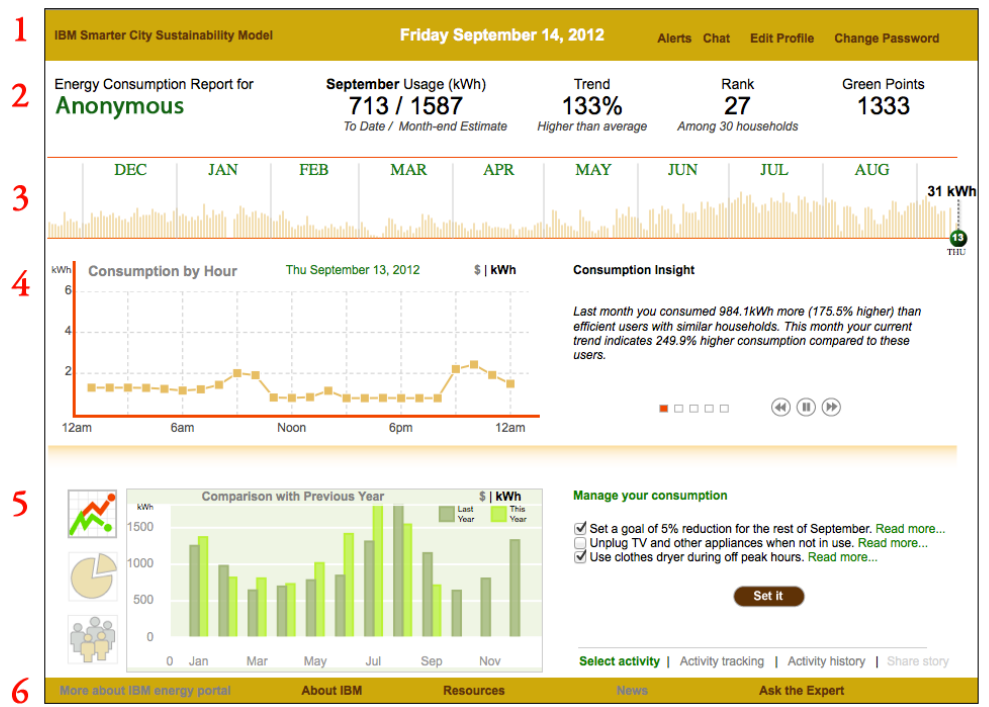
\includegraphics[scale=0.26]{./electricity_portal.png}
	\caption{The electricity portal divided in the 6 bands.}
	\label{fig:electricityportal}
\end{figure}

The user interface of the portal can be seen in Figure~\ref{fig:electricityportal}. It is divided into 6 bands:
\begin{enumerate}
\item Header, with date and menu access.
\item User name, usage to date, estimate of current month's usage and three incentives: trend (for self comparison), rank (among other households) and `green points', which can be collected with actions such as completing one's profile.
\item Daily electricity usage displayed in kWh or in dollar.
\item A graph of todays consumption and a textual comparison of the users electricity consumption.
\item A graph allowing users to view their energy usage compared to the previous year, broken down by load or compared to 30 similar households. It also has a component where users can view and set their goals.
\item Links to general information.
\end{enumerate}

The portal was made available 765 households in a few contiguous neighborhoods in the city of Dubuque in the United States and the project ran for about 20 weeks. Use of the portal was logged and surveys and interviews were held to find out about the experiences of the users of the portal.

%results
%  numbaahs
Out of 765 households, 266 (35\%) logged into the portal at least one time. In the survey, respondents were asked to estimate how often they used the portal. The responses were as follows:
\begin{enumerate}
\item five or more times per week -- 12\%
\item about once a week -- 18\%
\item occasional use -- 31\%
\item rare use -- 25\%
\item not applicable / do not recall -- 14\%
\end{enumerate}

In the survey, participants were also asked about the UI components whether they usually looked at them, if they needed more explanation, if it helped them to better understand their electricity consumption and if it encouraged them to undertake action. The responses in percentages to these questions can be seen in Table~\ref{uicomponents}. %TODO: consclusion based on table 7

The first four components, which are the most looked at are all time-based graphs/metrics. 

\begin{table}
  \caption{The UI components, ordered by popularity with the answers by participants to questions in percentages}
  \label{uicomponents}
  \scriptsize
  \begin{center}
    \begin{tabular}{lcccc}
    
        & \multicolumn{1}{p{1.2cm}}{\centering Usually looked at it} & 
        \multicolumn{1}{p{1.0cm}}{\centering Was entirely clear} & 
        \multicolumn{1}{p{1.3cm}}{\centering Helped to understand use} & 
        \multicolumn{1}{p{1.2cm}}{\centering Encouraged to act} \\ \hline
        
        \pbox{20cm}{Consumption\\ timeline} & 93\% & 53\% & 76\% & 49\% \\[0.25cm]
        \pbox{20cm}{Consumption\\ by hour} & 87\% & 53\% & 79\% & 52\% \\[0.25cm]
        \pbox{20cm}{Comparison with\\ previous year} & 87\% & 55\% & 58\% & 44\% \\[0.25cm]
        \pbox{20cm}{Monthly usage} & 81\% & 49\% & 58\% & 45\% \\[0.1cm]
        \pbox{20cm}{Consumption\\ insights} & 77\% & 38\% & 46\% & 47\% \\[0.25cm]
        \pbox{20cm}{Comparison \\with neighbor} & 67\% & 33\% & 30\% & 28\% \\[0.25cm]
        \pbox{20cm}{Consumption\\ by load} & 64\% & 40\% & 48\% & 31\% \\[0.20cm]
        \pbox{20cm}{Trend, Rank, Points} & 64\% & 32\% & 41\% & 44\% \\[0.05cm]
        \pbox{20cm}{Manage your\\ consumption} & 62\% & 46\% & 34\% & 35\% \\[0.1cm]
        \pbox{20cm}{Alerts} & 32\% & 33\% & 24\% & 19\% \\
		\pbox{20cm}{Facebook chat} & 10\% & 27\% & 1\% & 1\% \\
    \end{tabular}
  \end{center}
\end{table}

All 266 participating households reduced their electricity usage. Compared to electricity consumption of the previous year, they saved on average $31,817$ kWh during the project. This amounts to a monthly reduction of 3.7\%. In the survey, 69\% of the respondents indicated that the portal increased their understanding of how they consume electricity.

%\section{Results}
%The previous parts and the guidelines that some eco-feedbacks systems researches have established allow us to extract some requirements that the UI of eco-feedback should meet in order help the developers implementing softwares as effective as possible for the users. In the first subsection "famous" guidelines will be presented and in the second one the list of requirements. \\
%List of requirements : 
%Sustainability, Non-intrusiveness , Intuitiveness. Acceptability, Usability


\section{Conclusion}
In this paper, we looked at different user interface components used in eco-feedback systems. Based on several studies, we conclude that problems with understanding these interfaces for consumers are often caused by unfamiliarity with the scientific units used or how CO$_2$ relates to electricity usage. \\

Out of several studies, it can be concluded that interface components that present information in charts and tables are easily understood by consumers, especially when they concern time-based graphs/metrics. 
Most valued by consumers are UI components that present information about costs, per-device-breakdown of electricity usage and historical comparison.

It can also be concluded that using electricity usage information from peer networks can lead to more consistent energy saving when compared to only showing the users own electricity usage.

The use of incentives to motivate consumers to save electricity is also effective in making consumers use the eco-feedback system, especially when they start with a positive number of points.

\section{Future work}


%% if specified like this the section will be ommitted in review mode
%\acknowledgements{
%The authors wish to thank A, B, C. This work was supported in part by
%a grant from XYZ.}

\bibliographystyle{abbrv}
%%use following if all content of bibtex file should be shown
%\nocite{*}
\bibliography{template}
\end{document}
